\documentclass[10pt,twocolumn,letterpaper]{article}

\usepackage{cvpr}
\usepackage{times}
\usepackage{epsfig}
\usepackage{graphicx}
\usepackage{amsmath}
\usepackage{amssymb}
\usepackage{graphicx} % Allows you to include images
\usepackage{enumitem} % Allows customization of list spacing
\usepackage{float} % To control float positioning
\usepackage{placeins} % For FloatBarrier
\usepackage{booktabs}
\usepackage{multirow}
\usepackage{afterpage}
\usepackage{amssymb}

% Include other packages here, before hyperref.

% If you comment hyperref and then uncomment it, you should delete
% egpaper.aux before re-running latex.  (Or just hit 'q' on the first latex
% run, let it finish, and you should be clear).
%\usepackage[pagebackref=true,breaklinks=true,letterpaper=true,colorlinks,bookmarks=false]{hyperref}
\usepackage{hyperref}
\usepackage{cleveref} % For clever referencing


\cvprfinalcopy % *** Uncomment this line for the final submission

\def\cvprPaperID{****} % *** Enter the CVPR Paper ID here
\def\httilde{\mbox{\tt\raisebox{-.5ex}{\symbol{126}}}}

% Pages are numbered in submission mode, and unnumbered in camera-ready
%\ifcvprfinal\pagestyle{empty}\fi
\begin{document}

%%%%%%%%% TITLE
\title{Project Report : CS 7643}

\author{Girish Sharma\\
{\tt\small gsharma@gatech.edu}
% For a paper whose authors are all at the same institution,
% omit the following lines up until the closing ``}''.
% Additional authors and addresses can be added with ``\and'',
% just like the second author.
% To save space, use either the email address or home page, not both
\and
Matias Vizcaino \\
{\tt\small avizcaino3@gatech.edu}
\and
William Gleason\\
{\tt\small wgleason3@gatech.edu}
}

\maketitle
%\thispagestyle{empty}

%%%%%%%%% ABSTRACT
\begin{abstract}

   We evaluate adapters as a parameter efficient alternative to conventional fine-tuning methods for adapting a pre-trained models to out-of-domain tasks. We take a base model RoBERTa and second-phase pre-trained variations of it, and employ a dual approach: i) fine-tune the base model to perform a specific task, and ii) train adapter modules for the same task. We observe that adapters can achieve comparable performance to fine-tuning. A similar observation can be made even when the model undergoes a second-phase of task-adaptive pre-training before fine-tuning. Beyond comparable performance, adapters have significant benefits over fine-tuning, in terms of greatly reduced trainable parameters, ability to perform sequential training on tasks, and combining multiple adapters to create a single model capable of performing multiple tasks.
\end{abstract}

%%%%%%%%% BODY TEXT
\section{Introduction/Background/Motivation}

\subsection{Objective} We explore how traditional methods using fine-tuning compare to newer architectures using adapters in the context of transfer learning with pre-trained models for natural language tasks. We conduct a comparison across 4 types of pre-trained models that have been used before in other studies \cite{gururangan2020dont}. 1. A generic LLM, RoBERTa. 2. An LLM pre-trained on text in the domain of a task (DAPT). 3. An LLM pre-trained on the unlabeled data from a specific task (TAPT) 4. LLM pre-trained on both (DAPT + TAPT). 

Adapters are more lightweight, modular and composable than traditional fine-tuning methods. However, there may exist a performance penalty due to the reduced number of trainable parameters. This project looks at using parameter-efficient adapters for the RoBERTa transformer to achieve comparable performance to fine-tuning. Expanding from (Houlsby et al., 2019), our scope consists of two adapter configurations (Pfeiffer and Houlsby) imposed over tasks that contain specialized language and domains not extensively available in the base RoBERTa model. This allows us to assess if adapters can infuse knowledge efficiently, in a way that is comparable to Gururangan’s Task Adaptive Pretraining (TAPT) with small datasets related to two tasks in the Computer Science domain and one task for Biomedicine. Additionally, we evaluate the effectiveness of Adapter Fusion, a recently proposed multi-task learning architecture that aims to leverage multiple modular adapters using an attention layer. 

Throughout the study, we evaluate our models and compare them by the F1-Macro Score and the number of trainable parameters of their network, with specific focus on traditional fine-tuning, TAPT pre-training, and adapter methods. Albeit we focus on a small number of low-resource tasks ($<$ 5K records), the results support the potential of adapters as a parameter-efficient contestant to fine-tuning and as a viable alternative to TAPT for some use-cases, such as mid-sized ($>$ 3K) datasets.

\subsection{Current State} A common practice today is to start with a model pre-trained on a broad corpus of information (such as books, websites and other general domains) and then use fine-tuning to train the model for a particular task. If the task sits within a specific domain not originally covered by model, continued  pre-training can be done on specific unlabelled corpus. Once a baseline pre-trained model has been established, task specific heads are added as the final layers, which get co-trained with the baseline weights using task specific labeled data. Fine-tuning has been shown to be very effective at performing a given task.



\begin{table*}[h]
    \centering
    \begin{tabular}{ l r r r }
        \hline
        \textbf{Model} & \textbf{Parameter Counts} & \textbf{Parameters Trained} & \textbf{Percentage Trained} \\
        \hline
        RoBERTa and full fine-tuning & 124,650,246 & 124,650,246 & 100.00\% \\
        Pfeiffer Adapters & 126,777,759 & 2,127,513 & 1.71\% \\
        Houlsby Adapters & 127,672,287 & 3,022,041 & 2.42\% \\
        \hline
    \end{tabular}
    \caption{\textbf{Model Parameters and Training Percentage for Pre-Training, Fine-Tuning and Adapters}}
    \label{tab:model-parameters}
\end{table*}

\begin{itemize}
\item \textbf{Pre-Trained Models} like RoBERTa, a bidirectional encoder model, uses techniques like Masked Language Modeling (MLM) and Next Sentence Prediction (NSP) to learn a deep understanding of language structure and continuity. An optional second phase of pre-training \cite{gururangan2020dont} continues the process on new data using the same unsupervised learning objectives. The internal weights and embeddings of the model are shifted to better represent the vocabulary and patterns found in the new data. These processes are often quite demanding in terms of data and compute resources.

\item \textbf{Full Fine-Tuning} is then used retrain the entire model on the task data. While this would likely lead to the best performance, studies have shown that earlier layers of the pre-trained model generally learn broad semantic and syntactic features and those don’t really change for any given task. Limitations of fine-tuning include the need to store and share a complete set of weights for each task, and the requirement to train all tasks simultaneously to avoid catastrophic forgetting \cite{mccloskey1989catastrophic}.

\item \textbf{Variable Fine-Tuning} arises as a more efficient way to fine-tune. Researchers have shown that Parameter-Efficient-Fine-Tuning (PEFT) methods that focus only on a small proportion of model weights (original or new), while keeping the remaining weights frozen, can match the performance of traditional full fine-tuning methods \cite{houlsby2019parameter} and address some of their limitations, largely as they preserve much of the original knowledge while still adapting to new tasks. Some examples of PEFT methods include adapters, which are small neural modules that are added to the pre-trained model and trained only on the task data.
\end{itemize}

\subsection{Motivation}  
\label{sec.motivation}
Fine-tuning has several benefits as it allows to use the learned representations of large pre-trained models for specific tasks. However, it also has some drawbacks:

\begin{itemize}
    \item Fine-tuning involves training a large number of parameters for each task. For large models which can be 100s of MB, storing and sharing a complete set of weights for each task can limit multi-task applications.
    \item All tasks must be trained simultaneously, limiting scalability. Sequential fine-tuning for multiple tasks leads to catastrophic forgetting \cite{mccloskey1989catastrophic}
\end{itemize}
Adapters do not suffer from these drawbacks \cite{houlsby2019parameter}. The number of trained parameters is a tiny fraction compared to fine-tuning, significantly reducing the computational resources for fine-tuning as shown in \Cref{tab:model-parameters}. This is achieved through the use of bottleneck architecture, which involves downsizing the outputs of the previous layer, passing them through a non-linearity, and then upsizing them to match the inputs of the next layer. Additionally, adapters are modular as multiple adapters can be loaded onto the same base model to perform multiple tasks, eliminating the need for a copy of the base model for each task. Further, as they preserve the original model weights, they are more capable of maintaining the base model integrity and performance across tasks.

Adapter Fusion is an extension of the adapter architecture \cite{pfeiffer2020adapterfusion}. In Adapter Fusion, several trained adapters are combined in parallel, and an attention layer is added on top of the adapters to combine (fuse) them. Adapter fusion is then retrained on one of the original adapter’s tasks while updating the fusion layer and the classification head. We are interested in finding if this approach leads to better performance than a stand-alone adapter. Fusion allows the new model to leverage the original adapters information plus the potentially beneficial information from the other adapters without modifying their weights. This can lead to performance beyond just the original adapter while only minimally increasing the number of parameters. Additionally, by locking the base model and the adapter parameters the fusion setup avoids the problem of catastrophic forgetting that is typically an issue when fine tuning for multi-task training.

Gururangan et al. \cite{gururangan2020dont} highlights the benefits of domain-adaptive pre-training (DAPT) and task-adaptive pre-training (TAPT), which tailor the pre-training phase to more closely align with the characteristics of the target tasks, potentially enhancing subsequent fine-tuning outcomes. For instance, they expose low vocabulary overlap between RoBERTa and the domain of Computer Science, and find that continued pre-training on this domain is beneficial for related tasks. Their insights are crucial for informing more efficient strategies for effective task-specific tuning, although they rely on expensive methods of retraining and fine-tuning. In “Parameter-Efficient Transfer Learning for NLP” \cite{houlsby2019parameter}, the authors show that adapters attain within 0.4\% of the performance of full-fine-tuning, adding only 3.6\% parameters per task. The paper used the BERT transformer as its pre-trained model and used tasks from the GLUE benchmark to prove its assertions. 

We study parameter-efficient task adaptation using the RoBERTa model, which is a more robust version of BERT \cite{liu2019roberta}, and compare the results to those of Gururangan et al. \cite{gururangan2020dont}. As per Houlsby et al. \cite{houlsby2019parameter}, we expect the performance of adapters to be comparable to full fine-tuning, and further explore the capabilities for adapters as a viable alternative to TAPT to perform on out-of-domain tasks.

\begin{table*}[h]
    \centering
    \begin{tabular}{ l l l r r r r }
      \hline
      \textbf{Domain} & \textbf{Task} & \textbf{Label Type} & \textbf{Train} & \textbf{Dev}   & \textbf{Test}  & \textbf{Classes} \\
      \hline
      Computer Science & ACL-ARC & citation intent & 1,688 & 114   & 139   & 6 \\
                       & SCIERC  & relation classification & 3,219 & 455   & 974   & 7 \\
      \hline
      BIOMED           & CHEMPROT & relation classification & 4,169 & 2,427 & 3,469 & 13 \\
      \hline
    \end{tabular}%
    \caption{\textbf{Dataset Statistics}}
    \label{tab:dataset-stats}%
  \end{table*}%

%-------------------------------------------------------------------------
%------------------------------------------------------------------------
\section{Approach}
Our objective is to establish adapters as a suitable transfer learning approach for a given task, as compared with fine-tuning and task-adaptive pretraining methods. For this we recreate a fine-tuning the baseline that was used in the transfer learning paper \cite{gururangan2020dont}. We then take the four pre-trained models (RoBERTa base, DAPT, TAPT, DAPT-TAPT) per task and train adapters under two configurations, Pfeiffer and Houlsby. Our results are directly comparable to the original paper \cite{gururangan2020dont} and our own reproduction of their results.

\subsection{Data, Domain, and Tasks} 
We take data available to download by Allen Institute \cite{allenai_dont_stop_pretraining}. Our scope outlined in \Cref{tab:dataset-stats} is a subset of tasks from Gururanga et al. \cite{gururangan2020dont} that includes two tasks under the CS domain, ACL-ARC (citation-intent) and SCIERC (relation classification), and one task from BIOMED domain, CHEMPROT (relation classification) to test our hypothesis under a new domain. All these tasks have under 5,000 training records (i.e., low-resource) \footnote{Attempts were made to train on high-resource tasks, but due to computational demands, this was infeasible within our timeframe and is set as a future objective. We further exclude the low-resource NEWS task HYPERPARTISIAN as the test/validation dataset is very small and has only 2 classes - this leads to inconsistent results from \cite{allenai_dont_stop_pretraining} under our current set-up, again to be investigated as a future objective.}.

The task datasets have similar class distribution and are imbalanced, as shown in \Cref{fig:datasetbalance}. Therefore, we use the F1 score as our evaluation metric \footnote{Following \cite{gururangan2020dont}, we use macro-f1 for our CS tasks and micro-f1 for the CHEMPROT task}, which is a better measure for imbalanced datasets. The F1 score is the harmonic mean of precision and recall, and is a better measure for imbalanced datasets. Also, this is the same metric used in the original paper \cite{gururangan2020dont} so it allows for comparison of results.

\subsection{Methodology} 

\textbf{Base Models and Fine-Tuning} For reproduction, we first aimed to use the same set-up as in Gururangan et. al. \cite{allenai_dont_stop_pretraining} but encountered limitations on compatibility with newer packages and versioning. Therefore, we chose the widely used HuggingFace Transformers library \cite{transformers} for training our models. We load the pre-trained models from \cite{allenai_dont_stop_pretraining} made publicly available \ref{table:base_models}, and fine-tune by training a classification head in supervised manner using the same task-specific datasets and similar approach to Gururangan et. al. \cite{gururangan2020dont}. We were able to recreate results that are close-enough to the reference paper (better in some cases), but further efforts may be needed for closer replication and inspection of original process \footnote{Although benchmark fine-tuning results broadly align, there are some differences, likely due to differences in infrastructure, libraries used, and possibly unreported training parameters. Biggest relative difference is our F1 roberta-base for ACL-ARC at 66.34 while Gururangan’s is 63.00}. The F1 metric from our version of fine-tuning results is taken as a benchmark to assess the performance of adapter methods.

\begin{figure}[h]
    \centering 
    \includegraphics[width=0.45\textwidth]{resources/tmp_optuna_search.png}
    \caption{Illustration: Optuna Hyperparameter Search of combinations for roberta-base SCIERC Task (Houlsby)}
    \label{fig:optuna_search}
\end{figure}

\textbf{Adapters}  To assess the efficacy of adapter methods, we integrate task-specific adapters (and a prediction head) to each of the base models and train them separately using task-specific data. For training and managing configurations, we use AdapterHub \cite{adapterhub_overview} and two architectures: 
\begin{itemize}
\item Pfeiffer \cite{pfeiffer2020adapterhub} is a lightweight configuration that adds adapter modules between feed-forward layers. This minimally disrupts the base representations and maintains ability to generalize while adapting to new tasks. 
\item Houlsby \cite{houlsby2019parameter} can handle more complexity as it also adds adapters within the multi-head attention layers of each block. This allows the adapters to modulate both the attention outputs and feedforward operations, potentially offering more task-specific adaptation.
\end{itemize}
The \ref{sec:model_layers} shows examples of the adapter modules added to the model for both configurations. Note the bottleneck architecture of the adapter modules. We compare results under two scopes: direct fine-tuning comparison, and continued taks-adaptive pre-training comparison.

\textbf{Adapter Fusion} For each task we created a fusion “within” the same domain (the adapter for that task plus an adapter for the other task in the same domain) and a fusion “cross" with another domain (the original adapter for that domain plus a task outside that domain). To evaluate the impact of additional domain pre-training we analyze adapter fusion for both Roberta-base as well as the CS-Roberta. We also restricted the analysis to just the Pfeiffer Adapter.

\begin{figure}[h]
    \centering 
    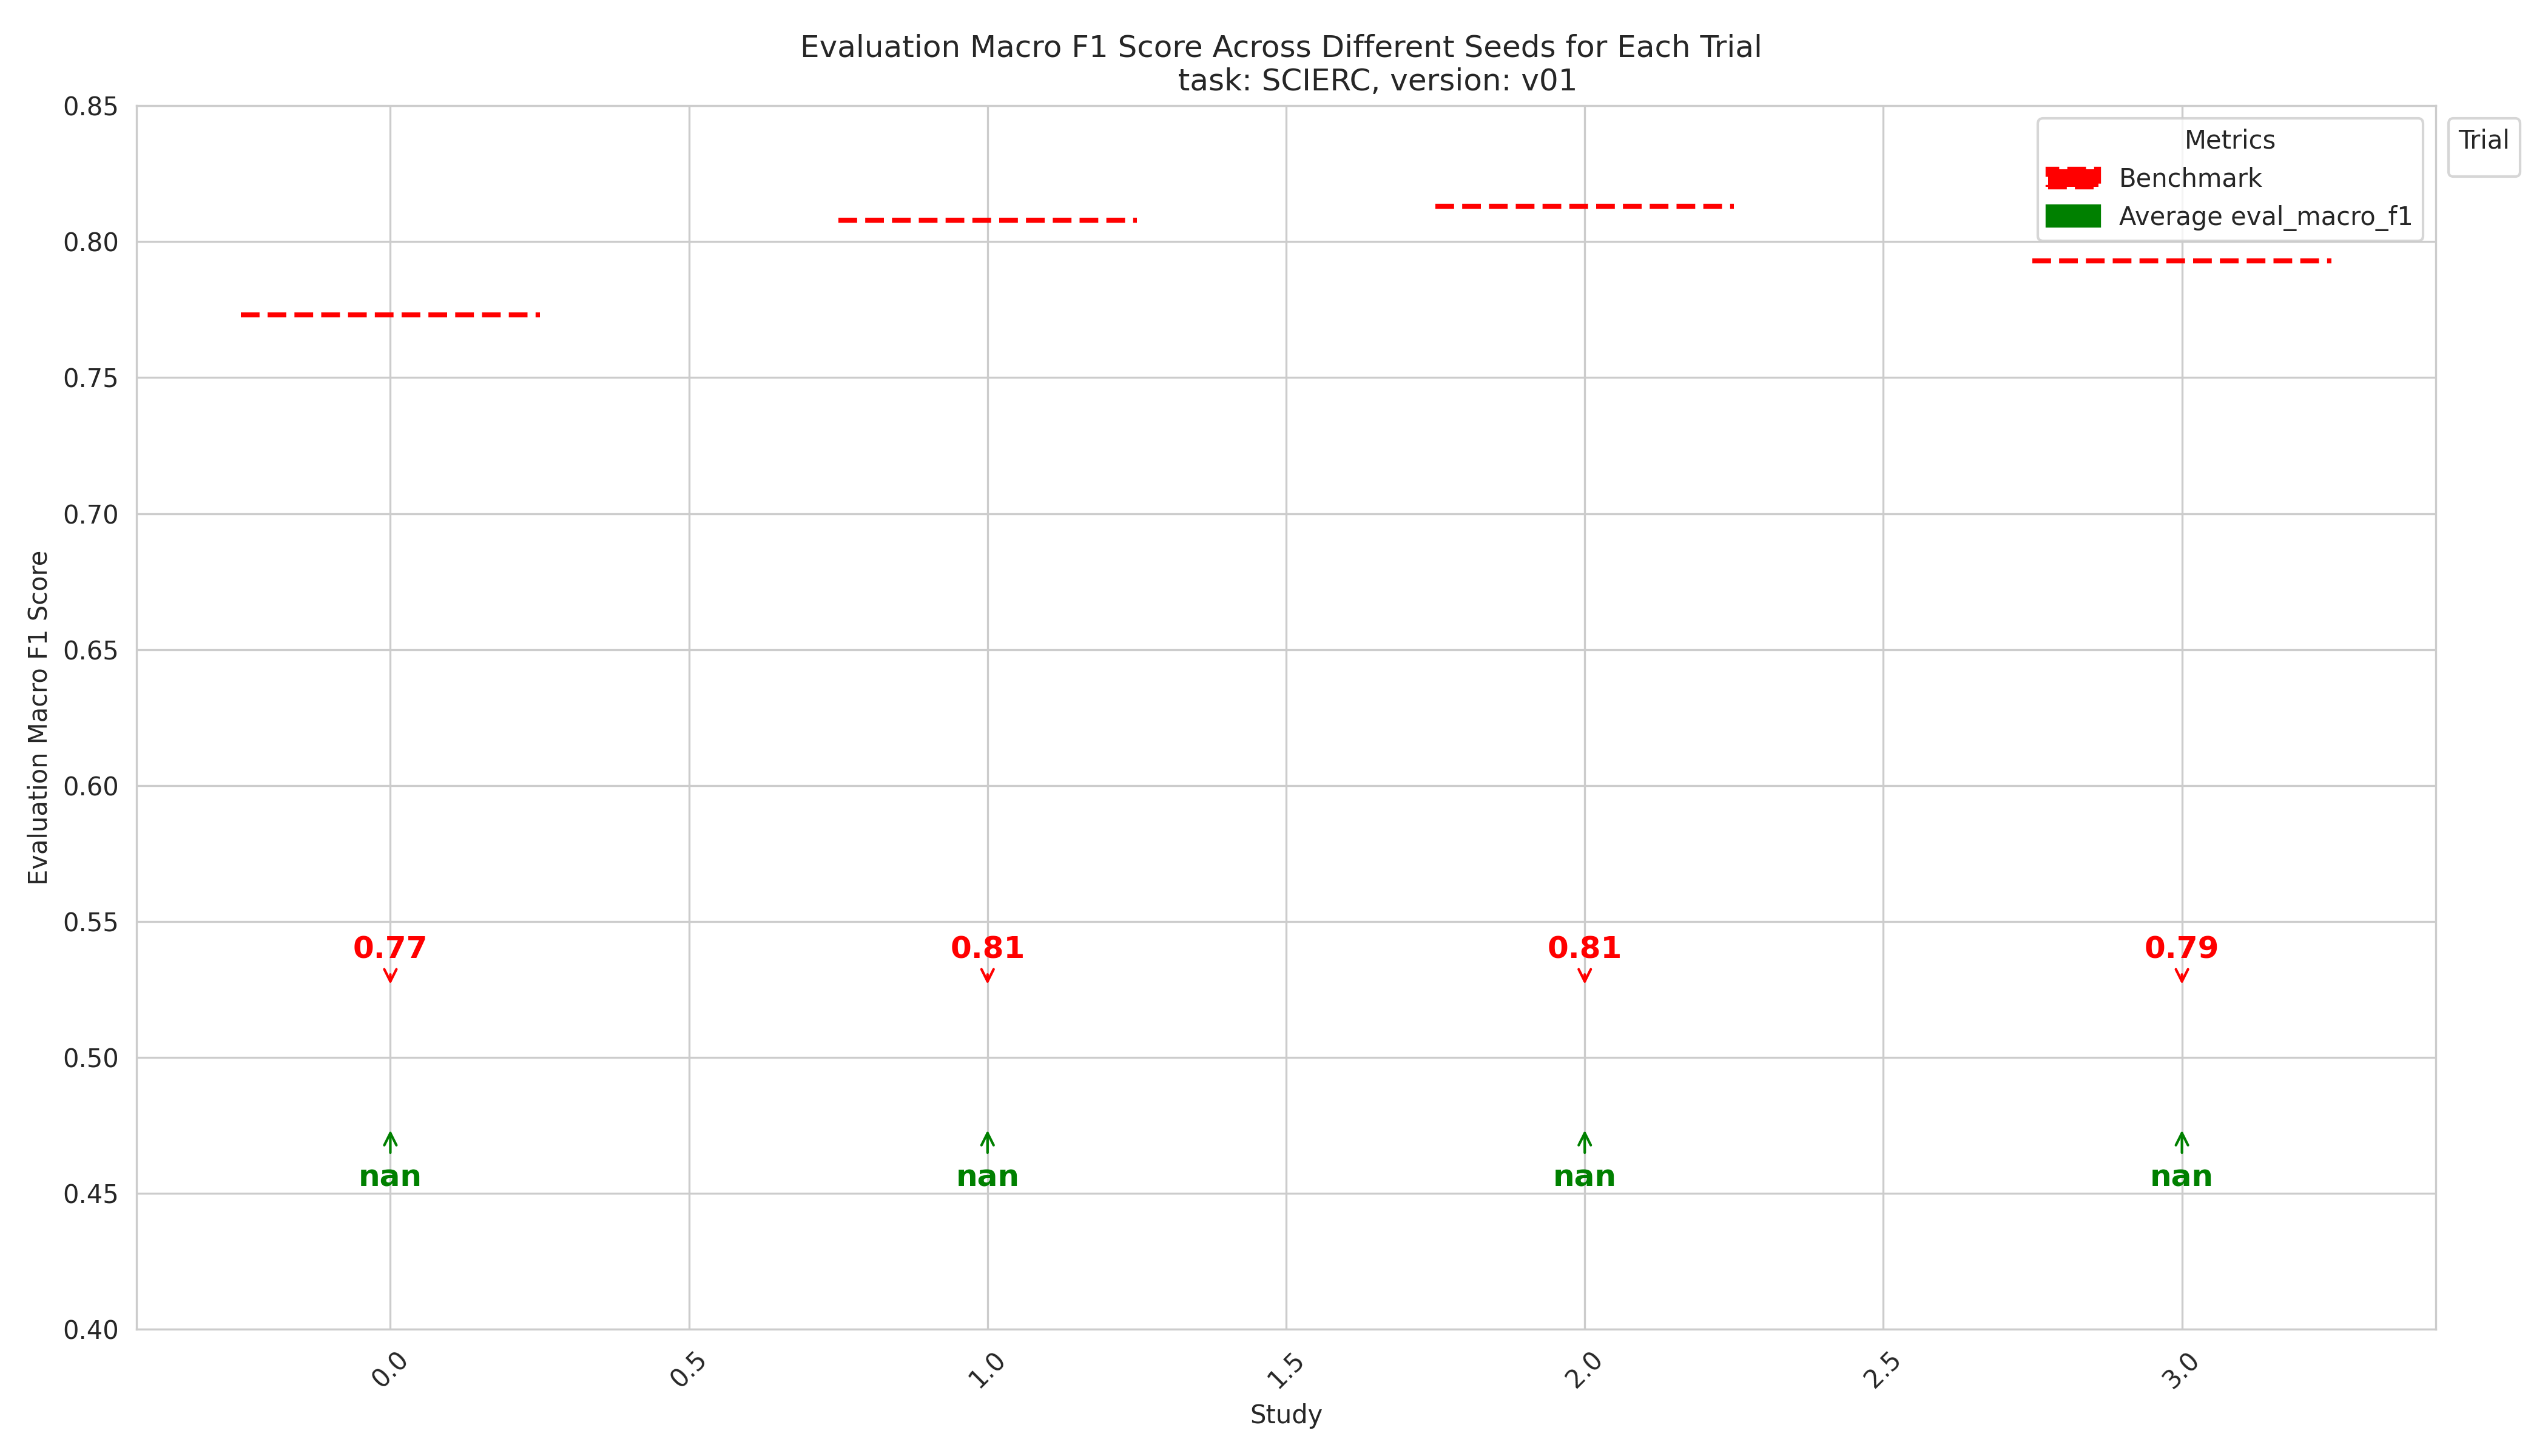
\includegraphics[width=0.45\textwidth]{resources/SCIERC/v01/evaluation_macro_f1_across_seeds.png}
    \caption{Illustration: Optuna trial results show convergence to good hyperparamer choices, other tasks follow similar patterns}
    \label{fig:optuna_search_trials}
\end{figure}

\subsection{Hyperparameter Search and Model Training} 

For training our adapters, by focusing on hyperparameter efficiency and robust training techniques, we achieved competitive results against traditional fine-tuning approaches, as detailed in our results from \Cref{table:aclarc} with configuration \ref{table:fine_tuning_hyperparameters}. Our approach demonstrates that adapters, when optimized properly, can effectively leverage pre-trained models for task-specific applications, and be on-par or surprass our baseline fine-tuning strategies.

\textbf{Hyperparameter Search:} Optuna \cite{optuna} was chosen as our hyperparameter optimization framework, especially useful in adapter training to traverse the combinations of learning rates, batch sizes and epochs. For a given search range \ref{table:optuna_search_space}, the framework applies Tree-Structured Parzen Estimator (TPE) that allowed for quick convergence to optimal settings, as illustrated in \Cref{fig:optuna_search_trials}. Each combination runs within a trial, and each trial is composed of 5 random seeds \footnote{The processes we ran also showed a lot of stochasticity across runs. We smoothed out most of the variance by the use of five random seeds, which helped in comparing across different runs. This is in line with \cite{allenai_dont_stop_pretraining} who report high standard deviation in their results, and also follow a 5-seed mean approach.}. The mean F1 on the test dataset is set as a performance metric for each trial, and we report this together with its standard deviation across the seeds. Smaller datasets often benefit from more granular updates (i.e., small batches) and moderate learning rattes prevent overfitting. Our best hyperparameters reflect this, as shown in \Cref{fig:optuna_search} and
\Cref{table:best_hyperparameters_adapters}. The number of training epochs does not show a clear correlation with the F1 score, as the models seem to require few iterations to capture task specifics.

\begin{figure}[h]
    \centering 
    \includegraphics[width=0.45\textwidth]{resources/SCIERC/v01/learning_curves_adapter.png}
    \caption{Example of Learning Curve convergence for roberta-base SCIERC Task (Houlsby) for the 5 seeds in best trial}
    \label{fig:learning_curve}
\end{figure}

\textbf{Training Optimization:} All models were trained using the Adam optimizer with L2 regularization, which is standard within the HuggingFace Transformers library. Since our tasks were all related to classification, cross-entropy loss was used for training. We adapted the learning rate and batch size based on outcomes from the Optuna search to maximize F1 score. Our experiments show robust performance across multiple training seeds, as shown in \Cref{fig:learning_curve}.

\begin{table*}[h]
    \centering
    \begin{tabular}{@{}lcc|lc|cc|@{}}
    \toprule
    \textbf{Pre-trained Model} & \multicolumn{2}{c}{Fine-Tuning} & \multicolumn{2}{c}{Adapters} & \multicolumn{2}{c}{Adapter Fusion} \\
    \cmidrule(lr){2-3} \cmidrule(lr){4-5} \cmidrule(lr){6-7}
    & Gururangan & Our Baseline & Pfeiffer & Houlsby & Within & Cross \\
    \midrule
    \multicolumn{1}{c}{\textbf{ACL-ARC}} \\
    ROBERTA & 63.00$_{\text{ 5.80}}$ & 66.34$_{\text{ 4.67}}$ & \textbf{67.12}$_{\text{ 1.85}}$ & 65.53$_{\text{ 1.30}}$ & \textit{73.30}\dag$_{\text{ 0.38}}$  & 72.35$_{\text{ 1.29}}$ \\
    TAPT & 67.40$_{\text{ 1.80}}$ & \textbf{69.49}$_{\text{ 2.24}}$ & 67.22$_{\text{ 3.92}}$ & 65.12$_{\text{ 1.22}}$ & & \\ 
    DAPT & \underline{75.40}$_{\text{ 2.50}}$ & \textbf{74.65}$_{\text{ 3.33}}$ & 73.32$_{\text{ 1.79}}$ & 74.03$_{\text{ 3.36}}$ & 73.59$_{\text{ 0.49}}$ & 74.06$_{\text{ 1.27}}$ \\ 
    DAPT\_TAPT & \underline{75.60}$_{\text{ 3.80}}$ & \textbf{74.89}$_{\text{ 2.48}}$ & 73.20$_{\text{ 2.84}}$ & 72.24$_{\text{ 1.55}}$ &  & \\ 
    \midrule
    \multicolumn{1}{c}{\textbf{SCIERC}} \\
    ROBERTA & 77.30$_{\text{ 1.90}}$ & 80.02$_{\text{ 1.20}}$ & \textbf{81.60}$_{\text{ 0.42}}$ & 81.32$_{\text{ 0.71}}$ & 80.32$_{\text{ 0.21}}$ & 80.32$_{\text{ 0.15}}$ \\ 
    TAPT & 79.30$_{\text{ 1.50}}$ & \textbf{80.95}$_{\text{ 0.74}}$ & 80.80$_{\text{ 1.35}}$ & 80.92$_{\text{ 0.76}}$ & & \\ 
    DAPT & 80.80$_{\text{ 1.50}}$ & \textbf{83.08}$_{\text{ 1.16}}$ & 82.48$_{\text{ 0.54}}$ & 82.55$_{\text{ 0.81}}$ & 81.64$_{\text{ 0.28}}$ & 81.53$_{\text{ 0.63}}$ \\ 
    DAPT\_TAPT & 81.30$_{\text{ 1.80}}$ & 81.55$_{\text{ 0.74}}$ & 81.47$_{\text{ 0.70}}$ & \textbf{88.81}$_{\text{ 0.58}}$ & & \\ 
    \midrule
    \multicolumn{1}{c}{\textbf{CHEMPROT}} \\
    ROBERTA & \underline{81.90}$_{\text{ 0.10}}$ & 80.69$_{\text{ 0.55}}$ & 80.38$_{\text{ 0.52}}$ & \textbf{80.95}$_{\text{ 0.40}}$ & & 80.55$_{\text{ 0.11}}$ \\ 
    TAPT & \underline{82.60}$_{\text{ 0.40}}$ & 79.88$_{\text{ 0.66}}$ & \textbf{80.80}$_{\text{ 0.45}}$ & 80.67$_{\text{ 0.65}}$ & & \\ 
    DAPT & \underline{84.20}$_{\text{ 0.20}}$ & 81.72$_{\text{ 0.41}}$ & 81.85$_{\text{ 0.51}}$ & \textbf{82.16}$_{\text{ 0.68}}$ & & \textit{82.77}\dag$_{\text{ 0.29}}$ \\ 
    DAPT\_TAPT & \underline{84.40}$_{\text{ 0.40}}$ & 81.71$_{\text{ 0.92}}$ & 81.67$_{\text{ 0.39}}$ & \textbf{82.29}$_{\text{ 0.40}}$ & & \\
    \bottomrule
    \end{tabular}
    \caption{\textbf{Comparison of Fine-tuning and Adapter Methods} We show baseline from the original paper \cite{gururangan2020dont} for reference but use our baseline for comparison with other methods. We further add results for Adapter Fusion, that is based on Pfeiffer adapters. Adapter Fusion was performed for within domain tasks (e.g., fuse ACL-ARC and SCIERC) and cross-domain tasks (e.g., fuse ACL-ARC and CHEMPROT). The best results are in bold (where \cite{gururangan2020dont} wins, its \underline{underlined}, where Adapter Fusion wins, it is in \textit{italics}\dag).}
    \label{table:aclarc}
\end{table*}

\subsection{Approach Remarks} 
Based on recent research showing the efficacy of adapters at performing on par with fine-tuning approaches \cite{houlsby2019parameter}, we felt confident that we can get comparable results with adapters. However, we take as baseline our reproduced results for fine-tuning as in \cite{gururangan2020dont}, which may not have been the best fine-tuning results possible for our tasks. We also note that the results of our fine-tuning are better than the original paper, which may be due to differences in infrastructure, libraries used, and possibly unreported training parameters.

Given the higher number of trainable parameters for adapters with Houlsby configuration, we expected Houlsby to have a better performance. Since we train on low-resource (small) datasets, the full benefits of the additional complexity of Houlsby may not be entirely realized in our experiments.



\section{Experiments and Results}

For our fine-tuning experiments, we add a classifier layer to the pre-trained models and co-train all the pre-trained weights and the classifier with the task data. For our adapters-based experiments, we add the adapters to the pre-trained models and the classification heads. We then train the adapters, which only trains the adapter layers and the final classification heads, without changing any of the pre-trained weights.

\subsection{Results}


\Cref{tab:model-parameters} shows the total parameter counts of the models when using fine-tuning and the adapters. Note that the Pfeiffer configuration is much more parameter-efficient than the Houlsby configuration, as it introduces fewer layers. A sample of the layers can be found in \ref{sec:model_layers}.



\subsection{Adapters vs Fine-Tuning} 

Based on our empirical results in \Cref{table:aclarc}, we see that both adapter configurations, Pfeiffer and Houlsby, were able to achieve on-par performance as full fine-tuning. The Pfeiffer configuration has an average difference of -0.33\% vs full fine-tuning and the Houlsby configuration shows a difference of 0.17\% \ref{table:adaptersvsft} \footnote{The Houlsby results have an outlier for SciERC and dapt\_tapt that performs 8.9\% better than fine-tuning. Future work will investigate this outlier for confirmation of results.}. This is in line with the results shown in other studies \cite{houlsby2019parameter}. The results clearly demonstrate the capacity of adapters to be as effective at transfer learning as full fine-tuning. The comparison of the models in \Cref{tab:model-parameters} also shows that the adapters needed just a fraction of the total parameters (1.71\% for Pfeiffer and 2.42\% for Houlsby) to be trained to achieve comparable results. 

This is quite a significant advantage of adapters, as they allow us to achieve the same results in transfer learning as full-fine-tuning, with just a tiny fraction of the trainable parameters needed for full fine-tuning. As discussed earlier, in \Cref{sec.motivation}, this was one of the motivations for this study.

\subsection{Adapters vs Continued Pre-Training} 

Adapters serve as both a complement to traditional fine-tuning and as a standalone alternative, offering targeted task optimization while reducing computational costs, which is especially beneficial in settings with limited resources.

\begin{table}[H]
    \centering
    \begin{tabular}{@{}lccccc@{}}
    \hline
    Base PT Model & TAPT & \multicolumn{2}{c}{Adapter} \\
    \cmidrule(lr){2-2} \cmidrule(lr){3-4}
    & & (Base) & (TAPT) \\
    \multicolumn{1}{c}{\textbf{ACL-ARC}} \\
    ROBERTA & \textbf{69.49}$_{\text{ 2.24}}$ & 67.12$_{\text{ 1.85}}$ & 67.22$_{\text{ 3.92}}$ \\
     DAPT & \textbf{74.89}$_{\text{ 2.48}}$ & 74.03*$_{\text{ 3.36}}$ & 74.03*$_{\text{ 3.36}}$ \\
    \hline
    \multicolumn{1}{c}{\textbf{SCIERC}}\\
    ROBERTA & 80.95$_{\text{ 0.74}}$ & \textbf{81.60}$_{\text{ 0.42}}$ & 80.92*$_{\text{ 0.76}}$ \\
    DAPT & 81.55$_{\text{ 0.74}}$ & 82.55*$_{\text{ 0.81}}$ & \textbf{88.81}*$_{\text{ 0.58}}$ \\
    \hline
    \multicolumn{1}{c}{\textbf{CHEMPROT}}\\
    ROBERTA & 79.88$_{\text{ 0.66}}\downarrow$ & \textbf{80.95}*$_{\text{ 0.40}}$ & 80.80$_{\text{ 0.45}}$ \\
    DAPT & 81.71$_{\text{ 0.92}}\downarrow$ & 82.16*$_{\text{ 0.51}}$ & \textbf{82.29}*$_{\text{ 0.40}}$ \\
\end{tabular}
\caption{\textbf{Adapters as an alternative to TAPT} The best results are in bold. Note that entries in the matrix that fall for both DAPT and TAPT have three phases of pre-training (base, DAPT and TAPT). For Adapters, where it includes a * it refers to Houlsby adapters, otherwise is Pfeiffer. A down arrow$\downarrow$ in TAPT indicates its the lowest score in the row.}
\label{table:adapters_vs_tapt}
\end{table}

From \Cref{table:adapters_vs_tapt} we further observe that using adapters without additional task-specific pre-training (as indicated by Adapter (Base)) provided comparable performance to using TAPT plus fine-tuning. This provides indication that, for some cases, adapters can serve as an alternative to TAPT, possibly due to an ability to infuse task-specific knowledge into the network throught the new layers. This is especially useful for low-resource tasks, where the cost of additional pre-training may not be justified. It's possible that TAPT may not provide as much benefit over adapters in our experiments since the task-specific terms may not be well-represented in the first phase pre-training corpus. Adapters allow for more targeted adjustments to the model, focusing specifically on the task-relevant aspects of the language without requiring extensive re-training of the model.



The experiments suggest that domain-specific pre-training (DAPT) provides a strong foundation for tasks within that domain, and adapters can effectively leverage and build upon this foundation. Adapters appear to be effective across different sizes of datasets. For smaller datasets, like ACL-ARC and SCIERC, they can provide the necessary specialization without extensive re-training. For larger datasets, such as CHEMPROT, adapters actually improve performance, indicating their utility across different scales of data availability.

\subsection{Pfeiffer vs Houlsby} 
Given the higher number of trainable parameters with Houlsby compared to Pfeiffer, we expected Houlsby configuration to perform better than Pfeiffer, in general. While the sample size of tasks is small to imply too broad a conclusion, we can see that for the chosen tasks and optimized training, the Houlsby configuration was slightly better than Pfeiffer, especially when the dataset is larger. When the datasets are small there is no discernible difference, as both configurations are equally capable of optimal learning. It is expected that Houlsby would be better generally, given the higher number of trained parameters introduced by the Houlsby configuration (2.42\% vs 1.71\%). However, Pfeiffer configuration does have a definite advantage of being more parameter-efficient and this would be a desirable quality when we are talking of lots of tasks. We could see a bit of tradeoff in parameter-efficient configuration vs task performance for bigger datasets.

\subsection{Adapter Fusion}
The “Within” adapter fusion results \ref{table:aclarc} were surprising for the ACL-ARC task. While the DAPT aligned with expectations, slightly exceeding that of the Pfeiffer adapter, the RoBERTa results far exceeded the adapter and were on par with DAPT. This could be because the training data of the SCI-ERC and was in the same domain, and so it was able to leverage some of that knowledge improve results.

The “Within” adapter fusion results for the SCI-ERC task performed slightly worse than the solo adapter. This could be for several reasons, the selection of the specific adapters 5 runs, the exact hyperparameters, or because the ACL-ARC adapter is not adding much value and so the additional values are leading to overfitting.

Finally, while the Cross Fusion results for SCIERC and CHEMPROT were close to expected, aligning producing similar results to the individual Pfeiffer Adapters, the results for ACL-ARC were surprising. Cross Adapter Fusion for RoBERTa performed almost on par with DAPT. This means the model gained significant information from adapter outside of its domain. This could be because of the large amount of training data for CHEMPROT and also because CHEMPROT’s Biomed domain has a 21\% overlap with the CS domain \cite{gururangan2020dont}


\section{Conclusions}
Through our experiments with natural language, low-resource tasks that extend beyond the original training domains of RoBERTa, we were able to demonstrate the capabilities of adapters to perform at par with fine-tuning alternatives for transfer learning tasks. While needing less than 3\% of the total trainable parameters as compared to fine-tuning, the adapters performance for the tasks matched full fine-tuning.

We also see that the benefits of pre-training across domain and tasks applied to adapters as well. Remarkably, adapters provided comparable or superior performance to TAPT, making them particularly valuable for low-resource settings with low budget or data availability for training. Additionally, through comparing the two popular adapter architectures – Pfeiffer and Houlsby, we find Houlsby performed slightly better when trained in our larger datasets, but the fact that Pfeiffer is more parameter-efficient and comparable to Houlsby in lower resource tasks makes it a competitive contestant. This is in line with expectations given Houlsby is naturally more adept for more complex tasks.

Adapter fusion shows promise as a method to improve results beyond a single adapter without significantly increasing the number of parameters, particularly when the domain or task of the adapters overlap.



Future work could explore additional adapter architectures, and their application across a wider range of NLP tasks and domains. We can also study the potential of Adapter Fusion to train on a completely new task.


%-------------------------------------------------------------------------
\onecolumn
\section{Appendix}

\appendix
\renewcommand{\thesection}{Appendix \Alph{section}}
\renewcommand{\thefigure}{\Alph{section}.\arabic{figure}}
\renewcommand{\thetable}{\Alph{section}.\arabic{table}}



\section{Team Members}
Our team was made up of three members. We all participated in periodic zoom calls where we discussed the technical details and work allocation of the project with equal participation from all.

\begin{table*}[h]
\begin{center}
\begin{tabular}{|l|c|p{8cm}|}
\hline
\textbf{Student Name} & \textbf{Contributed Aspects} & \textbf{Details} \\
\hline
Girish Sharma & Implementation and Analysis & Initial fine-tuning and adapter experiments with 5 seeds. Used manual hyper-parameter optimization. Comparison of Pfeiffer and Houlsby adapter architectures.  \\
Matias Vizcaino & Implementation and Analysis & Using Optuna-based hyper-parameter optimization for fine-tuning and adapter experiments. Created final results for fine-tuning and adapters, studied the potential of adapters as an alternative to TAPT. \\
William Gleason & Implementation and Analysis & Study of adapter composition using Adapter Fusion and other techniques. \\
\hline
\end{tabular}
\end{center}
\caption{\textbf{Contributions of team members.}}
\label{tab:contributions}
\end{table*}
\FloatBarrier


\section{Task Dataset Balance \& Illustration of Predictions}
% Insert a figure that spans both columns
\begin{figure*}[h] % 'h' suggests the figure appears in the specified location
    \centering % Center the image
    \includegraphics[width=0.60\textwidth]{./resources/label_distribution.png} % Make the image full page width
    \caption{Class Distribution for task datasets} % Add a caption
    \label{fig:datasetbalance} % Label the figure for cross-referencing
\end{figure*}

\begin{figure*}[h] % 'h' suggests the figure appears in the specified location
    \centering % Center the image
    \includegraphics[width=0.45\textwidth]{./resources/confusion_matrix_predictions_roberta-base_sciie_double_seq_bn.png} % Make the image full page width
    \caption{True vs Predicted labels for SciERC task using RoBERTa base model (Houlsby Adapter)} % Add a caption
    \label{fig:results} % Label the figure for cross-referencing
\end{figure*}
\FloatBarrier

\newpage{}
\section{HuggingFace Base Models Used}
The list below shows the pre-trained models used for the three tasks.

\begin{table}[h]
\centering
\begin{tabular}{lll}
\hline
\textbf{Task} & \textbf{Model Type} & \textbf{Downloaded from} \\ \hline
ACL-ARC & Base & roberta-base \\ 
 & DAPT & allenai/cs\_roberta\_base \\ 
 & TAPT & allenai/dsp\_roberta\_base\_tapt\_citation\_intent\_1688 \\ 
 & DAPT\_TAPT & allenai/dsp\_roberta\_base\_dapt\_cs\_tapt\_citation\_intent\_1688 \\ \hline
SciERC & Base & roberta-base \\ 
 & DAPT & allenai/cs\_roberta\_base \\ 
 & TAPT & allenai/dsp\_roberta\_base\_tapt\_sciie\_3219 \\ 
 & DAPT\_TAPT & allenai/dsp\_roberta\_base\_dapt\_cs\_tapt\_sciie\_3219 \\ \hline
CHEMPROT & Base & roberta-base \\ 
 & DAPT & allenai/biomed\_roberta\_base \\ 
 & TAPT & allenai/dsp\_roberta\_base\_tapt\_chemprot\_4169 \\ 
 & DAPT\_TAPT & allenai/dsp\_roberta\_base\_dapt\_biomed\_tapt\_chemprot\_4169 \\ \hline
\end{tabular}
\caption{Model Sources for Different Tasks}
\label{table:base_models}
\end{table}
\FloatBarrier

\section{Adapters vs Full FineTuning}
\begin{table}[h]
\centering

\begin{tabular}{llrrrrr}
\hline
\textbf{Dataset} & \textbf{Model} & \textbf{Fine-Tuning} & \textbf{Pfeiffer} & \textbf{Houlsby} & \textbf{Pfeiffer vs FT} & \textbf{Houlsby vs FT} \\
\hline
ACL-ARC & RoBERTA Base & 66.34 & 67.12 & 65.53 & 1.18\% & -1.22\% \\
& TAPT & 69.49 & 67.22 & 65.12 & -3.27\% & -6.29\% \\
& DAPT & 74.65 & 73.32 & 74.03 & -1.78\% & -0.83\% \\
& DAPT\_TAPT & 74.89 & 73.20 & 72.24 & -2.26\% & -3.54\% \\
\hline
SCIERC & RoBERTA Base & 80.02 & 81.60 & 81.32 & 1.97\% & 1.62\% \\
& TAPT & 80.95 & 80.80 & 80.92 & -0.19\% & -0.04\% \\
& DAPT & 83.08 & 82.48 & 82.55 & -0.72\% & -0.64\% \\
& DAPT\_TAPT & 81.55 & 81.47 & 88.81 & -0.10\% & 8.90\% \\
\hline
CHEMPROT & RoBERTA Base & 80.69 & 80.38 & 80.95 & -0.38\% & 0.32\% \\
& TAPT & 79.88 & 80.80 & 80.67 & 1.15\% & 0.99\% \\
& DAPT & 81.72 & 81.85 & 82.16 & 0.16\% & 0.54\% \\
& DAPT\_TAPT & 81.71 & 81.67 & 82.29 & -0.05\% & 0.71\% \\
\hline
\multicolumn{2}{l}{\textbf{Average}} & 77.91 & 77.66 & 78.05 & \textbf{-0.33\%} & \textbf{0.17\%} \\
\hline
\end{tabular}
\caption{Test accuracy for classification tasks across different pre-trained models. For each task and pre-trained model, the model with the best validation set accuracy is chosen. We report the mean test accuracy and s.e.m. across runs with
different random seeds.}
\label{table:adaptersvsft}
\end{table}

\newpage{}
\section{Training Environment and Hyper-Parameter Optimization}
\label{sec:besthyperparameters}

\begin{table}[H]

    \begin{minipage}[t]{0.45\textwidth}
    \centering
    \caption{Fine-Tuning Hyperparameters}
    \begin{tabular}{|l|l|}
    \hline
    \textbf{Hyperparameter} & \textbf{Value} \\
    \hline
    Number of Training Epochs & 10 \\
    Per-Device Training Batch Size & 16 \\
    Per-Device Evaluation Batch Size & 8 \\
    Learning Rate & $2 \times 10^{-5}$ \\
    Dropout & 0.1 \\
    \hline
    \end{tabular}
    \label{table:fine_tuning_hyperparameters}
    \end{minipage}
    \hfill
    \begin{minipage}[t]{0.45\textwidth}
    \centering
    \caption{Optuna Search Space}
    \begin{tabular}{|l|p{5cm}|}
    \hline
    \textbf{Parameter} & \textbf{Search Space} \\
    \hline
    Learning Rate & Loguniform distribution between $1 \times 10^{-5}$ and $1 \times 10^{-3}$ \\
    Batch Size & Discrete values: 16, 32, 64, 128 \\
    Number of Training Epochs & Uniform distribution between 5 and 15 (inclusive integers) \\
    \hline
    \end{tabular}
    \label{table:optuna_search_space}
    \end{minipage}
    
    \end{table}



\begin{table}[H]

    \centering
    \caption{Best Hyperparameters for Adapter Training Across Different Tasks}
    \begin{tabular}{@{}lcccc@{}}
    \hline
    \textbf{Study} & \textbf{Adapter} & \textbf{Learning Rate} & \textbf{Batch Size} & \textbf{Epochs} \\
    \hline
    \multicolumn{1}{c}{\textbf{ACL-ARC}} \\
    ROBERTA & Pfeiffer & 0.000793 & 16 & 15 \\
    ROBERTA & Houlsby & 0.000477 & 32 & 12 \\
    TAPT & Pfeiffer & 0.000983 & 32 & 11 \\
    TAPT & Houlsby & 0.000472 & 32 & 11 \\
    DAPT & Pfeiffer & 0.000581 & 32 & 14 \\
    DAPT & Houlsby & 0.000914 & 32 & 9 \\
    DAPT\_TAPT & Pfeiffer & 0.000332 & 16 & 14 \\
    DAPT\_TAPT & Houlsby & 0.000310 & 16 & 9 \\
    \hline
    \multicolumn{1}{c}{\textbf{SCIERC}} \\
    SCIERC
    ROBERTA & Pfeiffer & 0.000586 & 32 & 13 \\
    ROBERTA & Houlsby & 0.000953 & 32 & 9 \\
    TAPT & Pfeiffer & 0.000696 & 64 & 15 \\
    TAPT & Houlsby & 0.000628 & 16 & 13 \\
    DAPT & Pfeiffer & 0.000393 & 32 & 15 \\
    DAPT & Houlsby & 0.000973 & 16 & 13 \\
    DAPT\_TAPT & Pfeiffer & 0.000870 & 64 & 14 \\
    DAPT\_TAPT & Houlsby & 0.000994 & 16 & 13 \\
    \hline
    \multicolumn{1}{c}{\textbf{CHEMPROT}} \\
    ROBERTA & Pfeiffer & 0.000224 & 16 & 12 \\
    ROBERTA & Houlsby & 0.000588 & 16 & 11 \\
    TAPT & Pfeiffer & 0.000365 & 32 & 7 \\
    TAPT & Houlsby & 0.000346 & 16 & 9 \\
    DAPT & Pfeiffer & 0.000224 & 16 & 8 \\
    DAPT & Houlsby & 0.000396 & 16 & 5 \\
    DAPT\_TAPT & Pfeiffer & 0.000780 & 16 & 12 \\
    DAPT\_TAPT & Houlsby & 0.000857 & 16 & 9 \\
    \hline
    \end{tabular}
    \label{table:best_hyperparameters_adapters}
\end{table}

\FloatBarrier

\newpage{}
\section{Model layers}
\label{sec:model_layers}
Layers shown with parameter counts. Only showing the 1st layer for sample purposes. RoBERTa has 11 repeating layers. Note the difference between the Pfeiffer and Houlsby Adapters. Pfeiffer configuration adds adapter modules only between feed-forward layers. Houlsby configuration adds adapters within the multi-head attention layers of each block, in addition to the feed-forward layers. 

\begin{table}[htbp]
    \centering
    \small
    \caption{Description of Layers in Different Models}
    \begin{tabular}{|l|c|c|c|}
        \hline
        \textbf{Layer Description} & \textbf{RoBERTa Model} & \color{purple}\textbf{Pfeiffer Adapter} & \color{blue}\textbf{Houlsby Adapter} \\
        \hline
        \textbf{Repeating Layers} & & & \\
        roberta.embeddings.LayerNorm.bias & 768 & 768 & 768 \\
        roberta.encoder.layer.0.attention.self.query.weight & 589824 & 589824 & 589824 \\
        roberta.encoder.layer.0.attention.self.query.bias & 768 & 768 & 768 \\
        roberta.encoder.layer.0.attention.self.key.weight & 589824 & 589824 & 589824 \\
        roberta.encoder.layer.0.attention.self.key.bias & 768 & 768 & 768 \\
        roberta.encoder.layer.0.attention.self.value.weight & 589824 & 589824 & 589824 \\
        roberta.encoder.layer.0.attention.self.value.bias & 768 & 768 & 768 \\
        roberta.encoder.layer.0.attention.output.dense.weight & 589824 & 589824 & 589824 \\
        roberta.encoder.layer.0.attention.output.dense.bias & 768 & 768 & 768 \\
        roberta.encoder.layer.0.attention.output.LayerNorm.weight & 768 & 768 & 768 \\
        roberta.encoder.layer.0.attention.output.LayerNorm.bias & 768 & 768 & 768 \\
        \textbf{roberta.encoder.layer.0.output.adapters.adapter\_down.0.weight} & - & - & \color{blue}\textbf{36864} \\
        \textbf{roberta.encoder.layer.0.output.adapters.adapter\_down.0.bias} & - & - & \color{blue}\textbf{48} \\
        \textbf{roberta.encoder.layer.0.output.adapters.adapter\_up.weight} & - & - & \color{blue}\textbf{36864} \\
        \textbf{roberta.encoder.layer.0.output.adapters.adapter\_up.bias} & - & - & \color{blue}\textbf{768}\\
        roberta.encoder.layer.0.intermediate.dense.weight & 2359296 & 2359296 & 2359296 \\
        roberta.encoder.layer.0.intermediate.dense.bias & 3072 & 3072 & 3072 \\
        roberta.encoder.layer.0.output.dense.weight & 2359296 & 2359296 & 2359296 \\
        roberta.encoder.layer.0.output.dense.bias & 768 & 768 & 768 \\
        roberta.encoder.layer.0.output.LayerNorm.weight & 768 & 768 & 768 \\
        roberta.encoder.layer.0.output.LayerNorm.bias & 768 & 768 & 768 \\
        \textbf{roberta.encoder.layer.0.output.adapters.adapter\_down.0.weight} & - & \color{purple}\textbf{36864} & \color{blue}\textbf{36864} \\
        \textbf{roberta.encoder.layer.0.output.adapters.adapter\_down.0.bias} & - & \color{purple}\textbf{48} & \color{blue}\textbf{48} \\
        \textbf{roberta.encoder.layer.0.output.adapters.adapter\_up.weight} & - & \color{purple}\textbf{36864} & \color{blue}\textbf{36864} \\
        \textbf{roberta.encoder.layer.0.output.adapters.adapter\_up.bias} & - & \color{purple}\textbf{768} & \color{blue}\textbf{768}\\
        roberta.encoder.layer.1.attention.self.query.weight & 589824 & 589824 & 589824 \\
        \hline
        \textbf{Final Layers} & & & \\
        classifier.dense.weight & 589824 & - & - \\
        classifier.dense.bias & 768 & - & - \\
        classifier.out\_proj.weight & 4608 & - & - \\
        classifier.out\_proj.bias & 6 & - & - \\
        roberta.pooler.dense.weight & - & \color{purple}\textbf{589824} & \color{blue}\textbf{589824} \\
        roberta.pooler.dense.bias & - & \color{purple}\textbf{768} & \color{blue}\textbf{768} \\
        \textbf{heads.default.0.weight} & - & \color{purple}\textbf{589824} & \color{blue}\textbf{589824} \\
        \textbf{heads.default.0.bias} & - & \color{purple}\textbf{768} & \color{blue}\textbf{768} \\
        \textbf{heads.default.2.weight} & - & \color{purple}\textbf{768} & \color{blue}\textbf{768} \\
        \textbf{heads.default.2.bias} & - & \color{purple}\textbf{768} & \color{blue}\textbf{768} \\
        \textbf{heads.default.3.bias} & - & \color{purple}\textbf{50265} & \color{blue}\textbf{50265} \\
        \textbf{heads.base\_citation\_intent.1.weight} & - & \color{purple}\textbf{589824} & \color{blue}\textbf{589824} \\
        \textbf{heads.base\_citation\_intent.1.bias} & - & \color{purple}\textbf{768} & \color{blue}\textbf{768} \\
        \textbf{heads.base\_citation\_intent.4.weight} & - & \color{purple}\textbf{4608} & \color{blue}\textbf{4608} \\
        \textbf{heads.base\_citation\_intent.4.bias} & - & \color{purple}\textbf{6} & \color{blue}\textbf{6} \\
        \hline
    \end{tabular}
    \label{table:model_layers_table}
\end{table}





\section{Source Code}
Source code can be found at the following link:
\href{https://github.gatech.edu/avizcaino3/CS-7643-EfficiencyLane.git}{https://github.gatech.edu/avizcaino3/CS-7643-EfficiencyLane.git}

{\small
\bibliographystyle{ieee_fullname}
\bibliography{references}
}

\end{document}
